
%% bare_jrnl.tex
%% V1.4b
%% 2015/08/26
%% by Michael Shell
%% see http://www.michaelshell.org/
%% for current contact information.
%%
%% This is a skeleton file demonstrating the use of IEEEtran.cls
%% (requires IEEEtran.cls version 1.8b or later) with an IEEE
%% journal paper.
%%
%% Support sites:
%% http://www.michaelshell.org/tex/ieeetran/
%% http://www.ctan.org/pkg/ieeetran
%% and
%% http://www.ieee.org/

%%*************************************************************************
%% Legal Notice:
%% This code is offered as-is without any warranty either expressed or
%% implied; without even the implied warranty of MERCHANTABILITY or
%% FITNESS FOR A PARTICULAR PURPOSE! 
%% User assumes all risk.
%% In no event shall the IEEE or any contributor to this code be liable for
%% any damages or losses, including, but not limited to, incidental,
%% consequential, or any other damages, resulting from the use or misuse
%% of any information contained here.
%%
%% All comments are the opinions of their respective authors and are not
%% necessarily endorsed by the IEEE.
%%
%% This work is distributed under the LaTeX Project Public License (LPPL)
%% ( http://www.latex-project.org/ ) version 1.3, and may be freely used,
%% distributed and modified. A copy of the LPPL, version 1.3, is included
%% in the base LaTeX documentation of all distributions of LaTeX released
%% 2003/12/01 or later.
%% Retain all contribution notices and credits.
%% ** Modified files should be clearly indicated as such, including  **
%% ** renaming them and changing author support contact information. **
%%*************************************************************************


% *** Authors should verify (and, if needed, correct) their LaTeX system  ***
% *** with the testflow diagnostic prior to trusting their LaTeX platform ***
% *** with production work. The IEEE's font choices and paper sizes can   ***
% *** trigger bugs that do not appear when using other class files.       ***                          ***
% The testflow support page is at:
% http://www.michaelshell.org/tex/testflow/



\documentclass[journal]{IEEEtran}
%
% If IEEEtran.cls has not been installed into the LaTeX system files,
% manually specify the path to it like:
% \documentclass[journal]{../sty/IEEEtran}





% Some very useful LaTeX packages include:
% (uncomment the ones you want to load)


% *** MISC UTILITY PACKAGES ***
%
%\usepackage{ifpdf}
% Heiko Oberdiek's ifpdf.sty is very useful if you need conditional
% compilation based on whether the output is pdf or dvi.
% usage:
% \ifpdf
%   % pdf code
% \else
%   % dvi code
% \fi
% The latest version of ifpdf.sty can be obtained from:
% http://www.ctan.org/pkg/ifpdf
% Also, note that IEEEtran.cls V1.7 and later provides a builtin
% \ifCLASSINFOpdf conditional that works the same way.
% When switching from latex to pdflatex and vice-versa, the compiler may
% have to be run twice to clear warning/error messages.

\usepackage{outlines} % for bullets





% *** CITATION PACKAGES ***
%
%\usepackage{cite}
% cite.sty was written by Donald Arseneau
% V1.6 and later of IEEEtran pre-defines the format of the cite.sty package
% \cite{} output to follow that of the IEEE. Loading the cite package will
% result in citation numbers being automatically sorted and properly
% "compressed/ranged". e.g., [1], [9], [2], [7], [5], [6] without using
% cite.sty will become [1], [2], [5]--[7], [9] using cite.sty. cite.sty's
% \cite will automatically add leading space, if needed. Use cite.sty's
% noadjust option (cite.sty V3.8 and later) if you want to turn this off
% such as if a citation ever needs to be enclosed in parenthesis.
% cite.sty is already installed on most LaTeX systems. Be sure and use
% version 5.0 (2009-03-20) and later if using hyperref.sty.
% The latest version can be obtained at:
% http://www.ctan.org/pkg/cite
% The documentation is contained in the cite.sty file itself.






% *** GRAPHICS RELATED PACKAGES ***
%
\usepackage[pdftex]{graphicx}
\graphicspath{{./eps/}}
\graphicspath{{../../../3DSystem/DOC/wikiImages/}{./eps/}}
\DeclareGraphicsExtensions{.eps}

\ifCLASSINFOpdf
  \usepackage[pdftex]{graphicx}
  % declare the path(s) where your graphic files are
  % \graphicspath{{../pdf/}{../jpeg/}}
  % and their extensions so you won't have to specify these with
  % every instance of \includegraphics
  % \DeclareGraphicsExtensions{.pdf,.jpeg,.png}
\else
  % or other class option (dvipsone, dvipdf, if not using dvips). graphicx
  % will default to the driver specified in the system graphics.cfg if no
  % driver is specified.
  \usepackage[dvips]{graphicx}
  % declare the path(s) where your graphic files are
  \graphicspath{{./eps/}}
  % and their extensions so you won't have to specify these with
  % every instance of \includegraphics
  \DeclareGraphicsExtensions{.eps}
\fi
% graphicx was written by David Carlisle and Sebastian Rahtz. It is
% required if you want graphics, photos, etc. graphicx.sty is already
% installed on most LaTeX systems. The latest version and documentation
% can be obtained at: 
% http://www.ctan.org/pkg/graphicx
% Another good source of documentation is "Using Imported Graphics in
% LaTeX2e" by Keith Reckdahl which can be found at:
% http://www.ctan.org/pkg/epslatex
%
% latex, and pdflatex in dvi mode, support graphics in encapsulated
% postscript (.eps) format. pdflatex in pdf mode supports graphics
% in .pdf, .jpeg, .png and .mps (metapost) formats. Users should ensure
% that all non-photo figures use a vector format (.eps, .pdf, .mps) and
% not a bitmapped formats (.jpeg, .png). The IEEE frowns on bitmapped formats
% which can result in "jaggedy"/blurry rendering of lines and letters as
% well as large increases in file sizes.
%
% You can find documentation about the pdfTeX application at:
% http://www.tug.org/applications/pdftex





% *** MATH PACKAGES ***
%
\usepackage{amsmath}
% A popular package from the American Mathematical Society that provides
% many useful and powerful commands for dealing with mathematics.
%
% Note that the amsmath package sets \interdisplaylinepenalty to 10000
% thus preventing page breaks from occurring within multiline equations. Use:
%\interdisplaylinepenalty=2500
% after loading amsmath to restore such page breaks as IEEEtran.cls normally
% does. amsmath.sty is already installed on most LaTeX systems. The latest
% version and documentation can be obtained at:
% http://www.ctan.org/pkg/amsmath





% *** SPECIALIZED LIST PACKAGES ***
%
%\usepackage{algorithmic}
% algorithmic.sty was written by Peter Williams and Rogerio Brito.
% This package provides an algorithmic environment fo describing algorithms.
% You can use the algorithmic environment in-text or within a figure
% environment to provide for a floating algorithm. Do NOT use the algorithm
% floating environment provided by algorithm.sty (by the same authors) or
% algorithm2e.sty (by Christophe Fiorio) as the IEEE does not use dedicated
% algorithm float types and packages that provide these will not provide
% correct IEEE style captions. The latest version and documentation of
% algorithmic.sty can be obtained at:
% http://www.ctan.org/pkg/algorithms
% Also of interest may be the (relatively newer and more customizable)
% algorithmicx.sty package by Szasz Janos:
% http://www.ctan.org/pkg/algorithmicx




% *** ALIGNMENT PACKAGES ***
%
%\usepackage{array}
% Frank Mittelbach's and David Carlisle's array.sty patches and improves
% the standard LaTeX2e array and tabular environments to provide better
% appearance and additional user controls. As the default LaTeX2e table
% generation code is lacking to the point of almost being broken with
% respect to the quality of the end results, all users are strongly
% advised to use an enhanced (at the very least that provided by array.sty)
% set of table tools. array.sty is already installed on most systems. The
% latest version and documentation can be obtained at:
% http://www.ctan.org/pkg/array


% IEEEtran contains the IEEEeqnarray family of commands that can be used to
% generate multiline equations as well as matrices, tables, etc., of high
% quality.




% *** SUBFIGURE PACKAGES ***
%\ifCLASSOPTIONcompsoc
%  \usepackage[caption=false,font=normalsize,labelfont=sf,textfont=sf]{subfig}
%\else
%  \usepackage[caption=false,font=footnotesize]{subfig}
%\fi
% subfig.sty, written by Steven Douglas Cochran, is the modern replacement
% for subfigure.sty, the latter of which is no longer maintained and is
% incompatible with some LaTeX packages including fixltx2e. However,
% subfig.sty requires and automatically loads Axel Sommerfeldt's caption.sty
% which will override IEEEtran.cls' handling of captions and this will result
% in non-IEEE style figure/table captions. To prevent this problem, be sure
% and invoke subfig.sty's "caption=false" package option (available since
% subfig.sty version 1.3, 2005/06/28) as this is will preserve IEEEtran.cls
% handling of captions.
% Note that the Computer Society format requires a larger sans serif font
% than the serif footnote size font used in traditional IEEE formatting
% and thus the need to invoke different subfig.sty package options depending
% on whether compsoc mode has been enabled.
%
% The latest version and documentation of subfig.sty can be obtained at:
% http://www.ctan.org/pkg/subfig




% *** FLOAT PACKAGES ***
%
%\usepackage{fixltx2e}
% fixltx2e, the successor to the earlier fix2col.sty, was written by
% Frank Mittelbach and David Carlisle. This package corrects a few problems
% in the LaTeX2e kernel, the most notable of which is that in current
% LaTeX2e releases, the ordering of single and double column floats is not
% guaranteed to be preserved. Thus, an unpatched LaTeX2e can allow a
% single column figure to be placed prior to an earlier double column
% figure.
% Be aware that LaTeX2e kernels dated 2015 and later have fixltx2e.sty's
% corrections already built into the system in which case a warning will
% be issued if an attempt is made to load fixltx2e.sty as it is no longer
% needed.
% The latest version and documentation can be found at:
% http://www.ctan.org/pkg/fixltx2e


%\usepackage{stfloats}
% stfloats.sty was written by Sigitas Tolusis. This package gives LaTeX2e
% the ability to do double column floats at the bottom of the page as well
% as the top. (e.g., "\begin{figure*}[!b]" is not normally possible in
% LaTeX2e). It also provides a command:
%\fnbelowfloat
% to enable the placement of footnotes below bottom floats (the standard
% LaTeX2e kernel puts them above bottom floats). This is an invasive package
% which rewrites many portions of the LaTeX2e float routines. It may not work
% with other packages that modify the LaTeX2e float routines. The latest
% version and documentation can be obtained at:
% http://www.ctan.org/pkg/stfloats
% Do not use the stfloats baselinefloat ability as the IEEE does not allow
% \baselineskip to stretch. Authors submitting work to the IEEE should note
% that the IEEE rarely uses double column equations and that authors should try
% to avoid such use. Do not be tempted to use the cuted.sty or midfloat.sty
% packages (also by Sigitas Tolusis) as the IEEE does not format its papers in
% such ways.
% Do not attempt to use stfloats with fixltx2e as they are incompatible.
% Instead, use Morten Hogholm'a dblfloatfix which combines the features
% of both fixltx2e and stfloats:
%
% \usepackage{dblfloatfix}
% The latest version can be found at:
% http://www.ctan.org/pkg/dblfloatfix




%\ifCLASSOPTIONcaptionsoff
%  \usepackage[nomarkers]{endfloat}
% \let\MYoriglatexcaption\caption
% \renewcommand{\caption}[2][\relax]{\MYoriglatexcaption[#2]{#2}}
%\fi
% endfloat.sty was written by James Darrell McCauley, Jeff Goldberg and 
% Axel Sommerfeldt. This package may be useful when used in conjunction with 
% IEEEtran.cls'  captionsoff option. Some IEEE journals/societies require that
% submissions have lists of figures/tables at the end of the paper and that
% figures/tables without any captions are placed on a page by themselves at
% the end of the document. If needed, the draftcls IEEEtran class option or
% \CLASSINPUTbaselinestretch interface can be used to increase the line
% spacing as well. Be sure and use the nomarkers option of endfloat to
% prevent endfloat from "marking" where the figures would have been placed
% in the text. The two hack lines of code above are a slight modification of
% that suggested by in the endfloat docs (section 8.4.1) to ensure that
% the full captions always appear in the list of figures/tables - even if
% the user used the short optional argument of \caption[]{}.
% IEEE papers do not typically make use of \caption[]'s optional argument,
% so this should not be an issue. A similar trick can be used to disable
% captions of packages such as subfig.sty that lack options to turn off
% the subcaptions:
% For subfig.sty:
% \let\MYorigsubfloat\subfloat
% \renewcommand{\subfloat}[2][\relax]{\MYorigsubfloat[]{#2}}
% However, the above trick will not work if both optional arguments of
% the \subfloat command are used. Furthermore, there needs to be a
% description of each subfigure *somewhere* and endfloat does not add
% subfigure captions to its list of figures. Thus, the best approach is to
% avoid the use of subfigure captions (many IEEE journals avoid them anyway)
% and instead reference/explain all the subfigures within the main caption.
% The latest version of endfloat.sty and its documentation can obtained at:
% http://www.ctan.org/pkg/endfloat
%
% The IEEEtran \ifCLASSOPTIONcaptionsoff conditional can also be used
% later in the document, say, to conditionally put the References on a 
% page by themselves.




% *** PDF, URL AND HYPERLINK PACKAGES ***
%
\usepackage{url}
% url.sty was written by Donald Arseneau. It provides better support for
% handling and breaking URLs. url.sty is already installed on most LaTeX
% systems. The latest version and documentation can be obtained at:
% http://www.ctan.org/pkg/url
% Basically, \url{my_url_here}.


% *** Lee MISC PACKAGES ***
\usepackage{epstopdf}
\usepackage{gensymb}
\usepackage{textcomp}
\usepackage{mathtools}% http://ctan.org/pkg/mathtools
\usepackage{geometry} 
\usepackage{units}
\usepackage{authblk} % for author multiple affiliations
\usepackage[noend]{algpseudocode}
\usepackage{algorithm}
\usepackage[binary-units=true]{siunitx}
\sisetup{load-configurations = abbreviations}
\usepackage{enumitem}

% Custom commands
\newcommand{\argmax}[1]{\underset{#1}{\operatorname{arg}\,\operatorname{max}}\;}
\long\def\comment#1{}


% *** Do not adjust lengths that control margins, column widths, etc. ***
% *** Do not use packages that alter fonts (such as pslatex).         ***
% There should be no need to do such things with IEEEtran.cls V1.6 and later.
% (Unless specifically asked to do so by the journal or conference you plan
% to submit to, of course. )


% correct bad hyphenation here
\hyphenation{op-tical net-works semi-conduc-tor}


\begin{document}
%
% paper title
% Titles are generally capitalized except for words such as a, an, and, as,
% at, but, by, for, in, nor, of, on, or, the, to and up, which are usually
% not capitalized unless they are the first or last word of the title.
% Linebreaks \\ can be used within to get better formatting as desired.
% Do not put math or special symbols in the title.
\title{Multi-ANN Edge System based on a Custom 3DIC DRAM}
%
%
% author names and IEEE memberships
% note positions of commas and nonbreaking spaces ( ~ ) LaTeX will not break
% a structure at a ~ so this keeps an author's name from being broken across
% two lines.
% use \thanks{} to gain access to the first footnote area
% a separate \thanks must be used for each paragraph as LaTeX2e's \thanks
% was not built to handle multiple paragraphs
%
\author{{Lee B. Baker, Paul Franzon~\IEEEmembership{Fellow,~IEEE}}%

\thanks{L. B. Baker, and P. Franzon are with the Department of Electrical and Computer Engineering,
North Carolina State University,
2410 Campus Shore Dr., Raleigh NC 27606 
Tel/Fax:
919-515-5460/5523
Email: 
lbbaker@ncsu.edu,
jasteve4@ncsu.edu,
paulf@ncsu.edu}

\thanks{Manuscript received Month Day, 2016; revised Month Day, 2016.}}

% note the % following the last \IEEEmembership and also \thanks - 
% these prevent an unwanted space from occurring between the last author name
% and the end of the author line. i.e., if you had this:
% 
% \author{....lastname \thanks{...} \thanks{...} }
%                     ^------------^------------^----Do not want these spaces!
%
% a space would be appended to the last name and could cause every name on that
% line to be shifted left slightly. This is one of those "LaTeX things". For
% instance, "\textbf{A} \textbf{B}" will typeset as "A B" not "AB". To get
% "AB" then you have to do: "\textbf{A}\textbf{B}"
% \thanks is no different in this regard, so shield the last } of each \thanks
% that ends a line with a % and do not let a space in before the next \thanks.
% Spaces after \IEEEmembership other than the last one are OK (and needed) as
% you are supposed to have spaces between the names. For what it is worth,
% this is a minor point as most people would not even notice if the said evil
% space somehow managed to creep in.



% The paper headers
\markboth{IEEE Transactions on Neural Networks and Learning Systems,~Vol.~XX, No.~XX, Month~2016}%
{Shell \MakeLowercase{\textit{et al.}}:Custom 3D-DRAM based ANN Edge System }
% The only time the second header will appear is for the odd numbered pages
% after the title page when using the twoside option.
% 
% *** Note that you probably will NOT want to include the author's ***
% *** name in the headers of peer review papers.                   ***
% You can use \ifCLASSOPTIONpeerreview for conditional compilation here if
% you desire.




% If you want to put a publisher's ID mark on the page you can do it like
% this:
%\IEEEpubid{0000--0000/00\$00.00~\copyright~2015 IEEE}
% Remember, if you use this you must call \IEEEpubidadjcol in the second
% column for its text to clear the IEEEpubid mark.



% use for special paper notices
%\IEEEspecialpapernotice{(Invited Paper)}




% make the title area
\maketitle

% As a general rule, do not put math, special symbols or citations
% in the abstract or keywords.
\begin{abstract}

Machine Learning in the form of Deep Neural Networks (DNN) have gained traction over the last few years.
They get good press in applications such as image recognition and speech recognition.
DNNs are constructed from a basic building block, the artificial neuron(AN).
With popular DNNs, the artificial neural network (ANN) is often formed from tens of layers of ANs with each layer containing many ANs.
In most cases, these layers are processed in a feed-forward manner with one layer being the inputs to the next layer.
Therefore, useful DNNs often require hundreds of thousands of ANs and within the network, each AN can have hundreds, even thousands of feeder or pre-synaptic ANs.

There have been implementations that use different number formats from double precision floating to eight bit integers, but in all cases these useful ANNs require significant
memory requirements to store the connection weights (parameters) therefore requiring Dynamic Random Access memory (DRAM) to store the AN parameters.

There have been many successful attempts to accelerate ANNs, but in most cases the focus is on a subset of the DNN known as the Convolutional Neural network (CNN).
CNNs assume a significant amout of reuse of the weights connecting ANs and thus they can take advantage of local memory (SRAM).

Much of the NN application specific (ASIC/ASIP) research has focused on taking advantage of the performance and ease of use of Static Random Access Memory (SRAM).
These implementations can be shown to be effective with specific NN architectures, such as CNNs where the ANN parameters can be stored in SRAM in a cache-like architecture avoiding constant accessing of the "slower" DRAM.
In addition, to achieve a high performance, these rely on processing a batch of inputs, such as processing a batch of images or voice recordings using the same ANN.

The work in this paper considers applications that require the processing of a disparate set of useful sized ANNs. The work assumes that the application system is utilizing ANNs
for the processing of various sub-systems, such as navigation, engine monitoring etc.. This work also does not assume the ANN is specifically a CNN but a DNN where there may
not be opportuities to store portions of the ANN in SRAM. This also includes no opportunities to perform batch processing.

This work uses the DRAM as the primary processing storage and employs minimal or no SRAM for the processing of the AN.
In additon, the work considers 3D integrated circuit technology and a custom 3D-DRAM. By employing 3DIC technology, this work takes advantage of the reduced energy and area and increased
connectivity and bandwidth to allow the DRAM to be employed efficiently without the need for local SRAM.
It should be noted that this work does not design a custom 3D-DRAM but answers the question "if such a device were available, can we employ it within a useful ANN system".


\end{abstract}

% Note that keywords are not normally used for peerreview papers.
\begin{IEEEkeywords}
machine learning, edge system, DNN, CNN, neural network
\end{IEEEkeywords}






% For peer review papers, you can put extra information on the cover
% page as needed:
% \ifCLASSOPTIONpeerreview
% \begin{center} \bfseries EDICS Category: 3-BBND \end{center}
% \fi
%
% For peerreview papers, this IEEEtran command inserts a page break and
% creates the second title. It will be ignored for other modes.
\IEEEpeerreviewmaketitle



\section{Introduction}
% The very first letter is a 2 line initial drop letter followed
% by the rest of the first word in caps.
% 
% form to use if the first word consists of a single letter:
% \IEEEPARstart{A}{demo} file is ....
% 
% form to use if you need the single drop letter followed by
% normal text (unknown if ever used by the IEEE):
% \IEEEPARstart{A}{}demo file is ....
% 
% Some journals put the first two words in caps:
% \IEEEPARstart{T}{his demo} file is ....
% 
% Here we have the typical use of a "T" for an initial drop letter
% and "HIS" in caps to complete the first word.
\IEEEPARstart{U}{seful} DNNs often require hundreds of thousands of ANs.
Within the network, each AN can have hundreds of feeder (pre-synaptic) ANs.
With popular DNNs, there are often tens of layers. 
So in these ANNs, the memory requirements are significant. The storage is required for the input, the AN state and most significantly the weights for each of the ANs. This storage requirement often results in gigabytes of memory.

When these ANNs are required to be solved in fractions of a second, the processing and memory bandwidth becomes prohibitive.

In most cases, Graphics processing Units (GPU) are used to implement large NNs. In many NN architectures, such as Convolutional NNs (CNN), they are quite effective. However, we should not forget they are not optimized purely for 
NN processing and are restricted by available SRAM and they are power hungry. These limitations will limit the effectiveness of GPUs regardless of what we might hear from the GPU community ("declare an interest").

Much of the NN application specific (ASIC/ASIP) research has focused on taking advantage of the performance and ease of use of Static Random Access Memory or SRAM. 
These implementations can be shown to be effective with specific NN architectures (CNN), server applications or the "toy examples" but when a system requires multiple disparate ANNs in an edge application, 
these implementations do not provide the required flexibility, storage capacity and deterministic performance.

Another technology that has been considered over the last decade is 3D integrated circuit technology (3DIC). 
This 3DIC technology stacks multiple die together to form a system-on-chip with potentially disparate technology for each die in the stack.
By staying within the die footprint, 3DIC technology promises high connectivity and consequently high bandwidth along with lower power all within a smaller footprint.

This work demonstrates a system that is able implement multiple useful sized DNNs whilst staying within the die stack footprint of a typical 3DIC DRAM.
This work also removes a reliance on SRAM to achieve high performance thus allowing the proposed design to be utilized in edge applcations when processing multiple disparate ANNs at or near real-time.
Although not optimized for specific ANNs, such as CNNs, this work demonstrates the potential for real-time performance when implementing fully connected DNNs or other such ANNs such as LSTM, at the edge.


% >>>>>>>>>>>>>>>>>>>>>>>>>>> System Description <<<<<<<<<<<<<<<<<<<<<<
\section{System Description}
\label{System Description}

% #######################################################################################################################################
% >>>>>>>>>>>>>>>>>>>>>>>>>>> Data Capture Hardware System <<<<<<<<<<<<<<<<<<<<<<
\subsection{ANN System}
\label{sec:ANN System}

The primary objectives of this work was to a) consider systems that are unable to take advantage of memory reuse opportunities and therefore not able to achieve high performance using
local SRAM to store ANN parameters or the ANN input, b) acknowedge that DRAM is required for storage of ANN parameters and c) that many edge devices will likely apply many disparate ANNs
to perform various system functions, and d) it is assumed that many edge applications will have space and power limitations.

These requirements suggest that reuse opportunities will not provide significant performance boosts and therefore this work focused on using the DRAM directly as the operational
storage and not rely on a significant amount of local SRAM.
This work employs 3DIC technology along with a custom 3D-DRAM. The objective was to demonstrate that a pure 3DIC system can implement multiple disparate ANNs. By staying within the 3DIC footprint and taking advantage of high
density through-silicon-vias (TSV) this work is able to maintain a significantly higher bandwidth over 2D or 2.5D solutions.

The 3DIC system die stack (figure \ref{fig:3DICStack}) includes the 3D-DRAM with a system manager below and one or more processing layers below the manager.
\begin{figure}[!t]
% the [] contains position info e.g. [!t] means here
\centerline{
\mbox{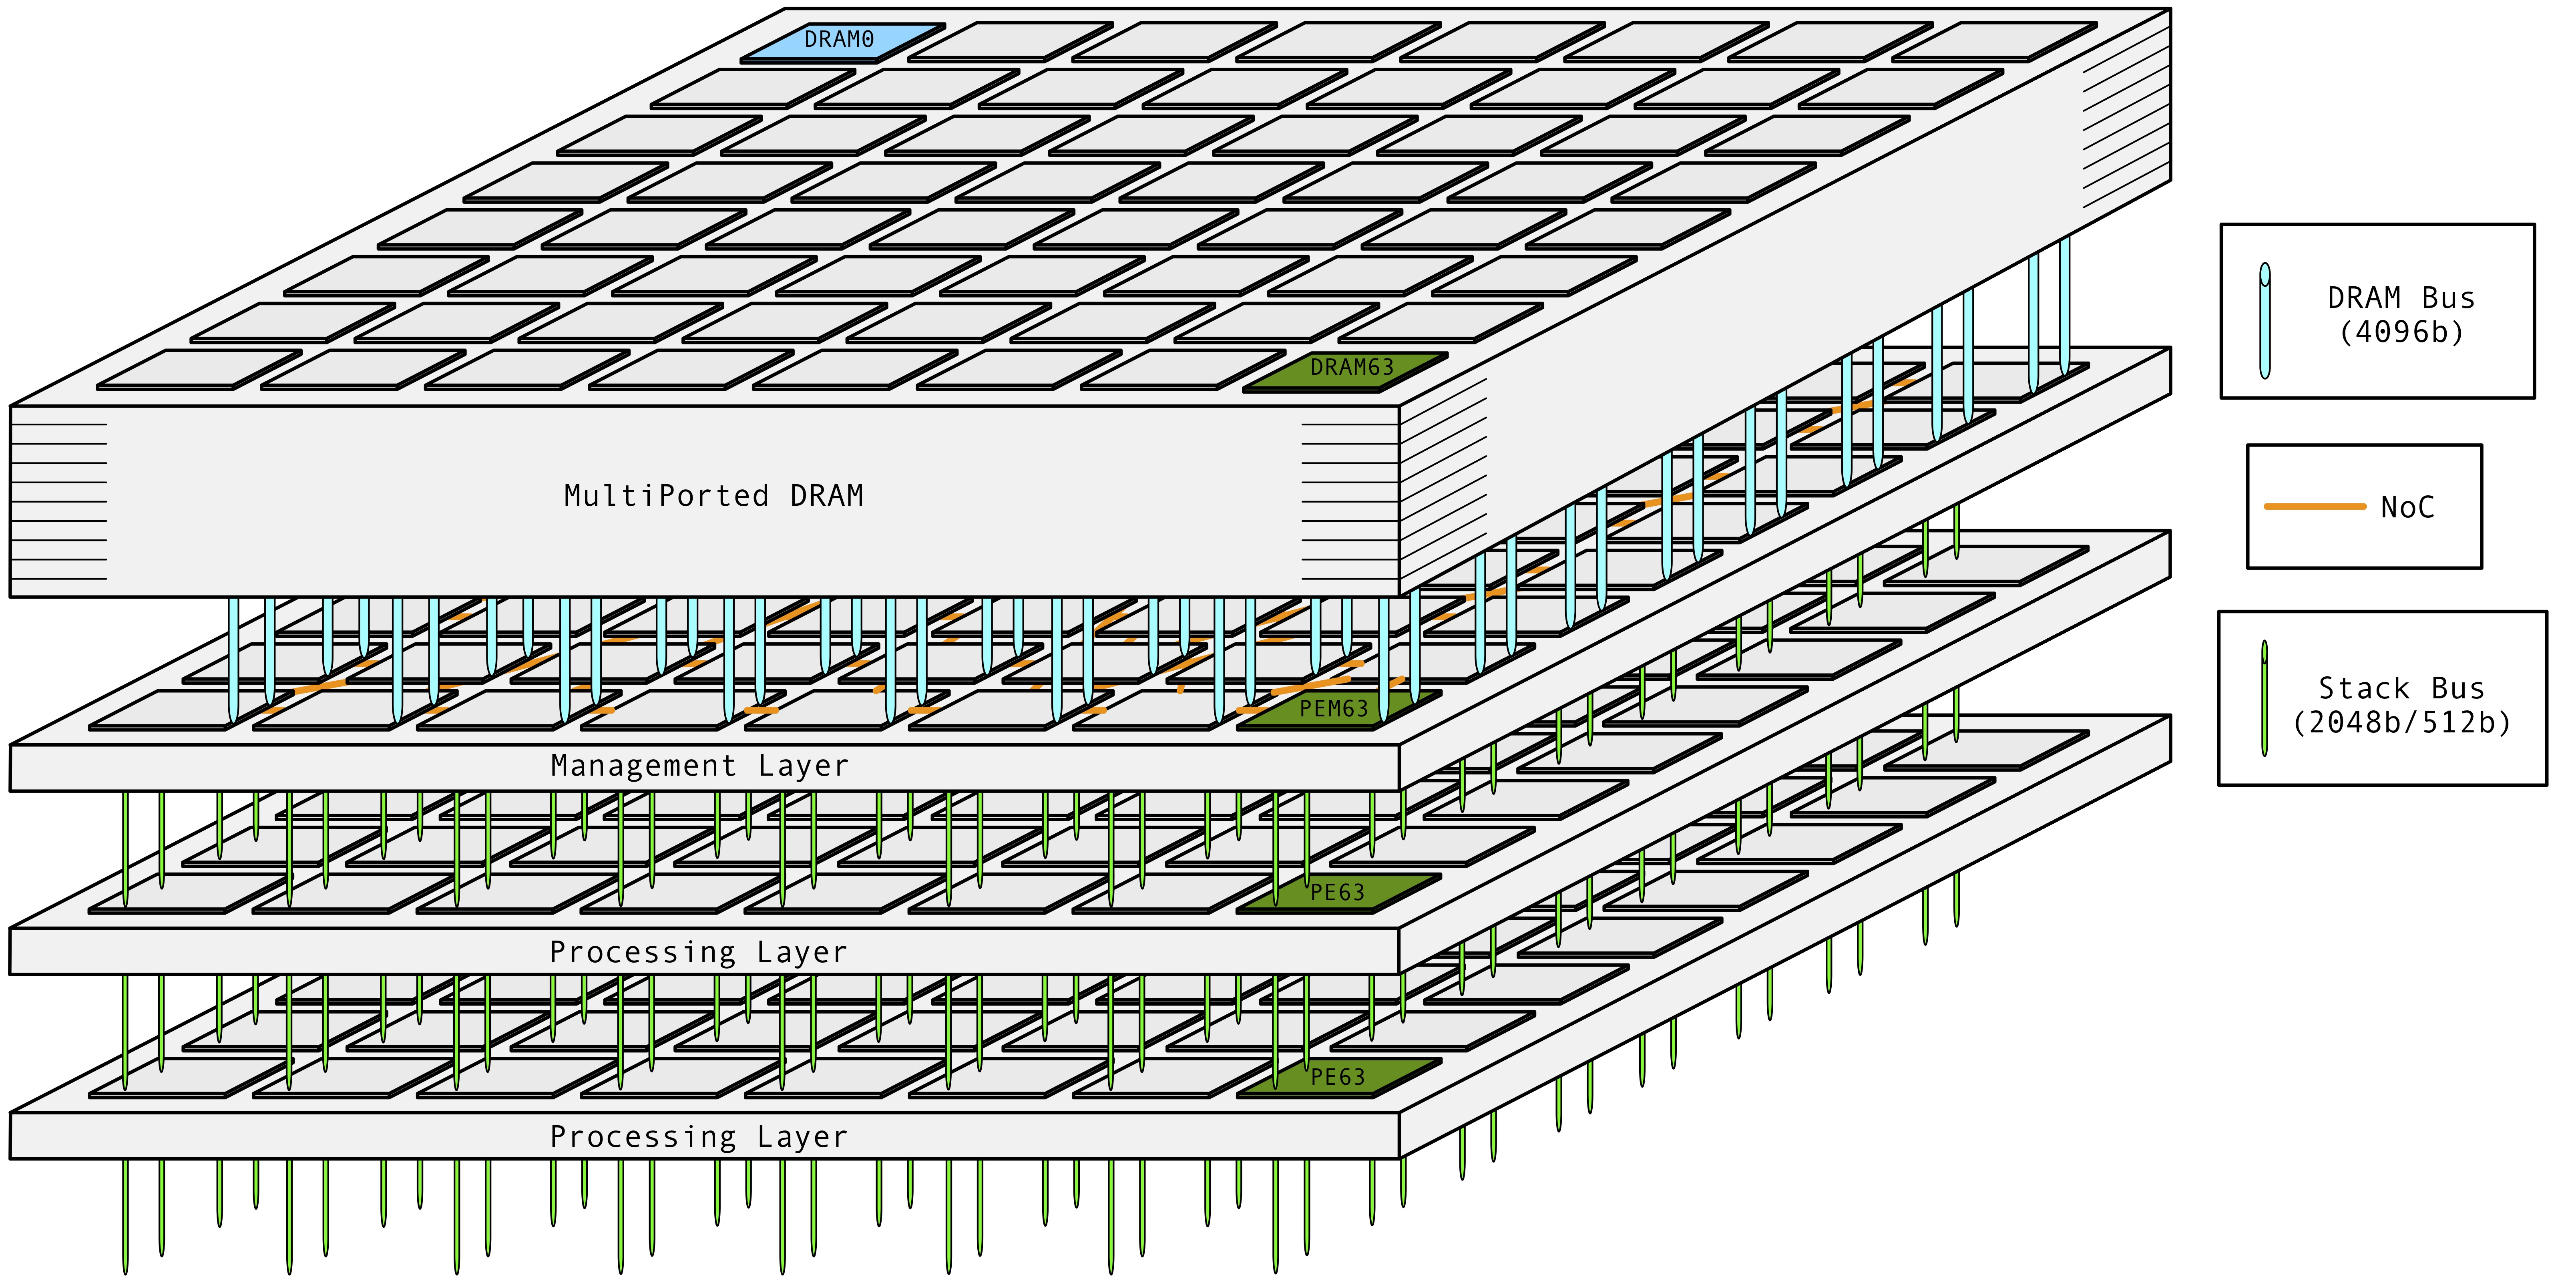
\includegraphics[width=2.5in]{StackDiagram.jpg}}
}
\caption{3DIC System Stack}
\label{fig:3DICStack}
\end{figure}

3D-DRAM has recently become available in standards such as High Bandwidth Memory (HBM) and Hybrid Memory Cube (HMC) and proprietary devices such as the DiRAM4 available from Tezzaron. 
These technologies provide high capacity within a small footprint.

In the case of HBM and DiRAM4, the technology can be combined with additional custom layers to provide a system solution.

The question becomes, can a useful system coexist within the same 3D footprint?

This work targeted a baselne system with:
\begin{itemize}
  \itemsep0em 
  \item target single precision floating point for computations
  \item use the Tezzaron DiRAM4 DRAM for area estimates and memory controller design
\end{itemize}
The work includes customizing the interface to the 3D-DRAM, researching data structures to describe storage of ANN parameters, designing a memory manager with micro-coded instructions and a processing engine (PE) layer.
The system is designed such that a sub-system, known as a system column operates on one of these disjoint memoriies within the 3D-DRAM. The sub-systems pass data using a network-on-chip (NoC).
An overview of the various blocks and interconnects are given below:

\subsubsection{3D-DRAM}
The targetted 3D-DRAM, the Tezzaron DiRAM4 is a 3D-DRAM employs multiple memory array layers in conjunction with a control and IO layer.
The memory is formed from 64 disjoint sub-memories each providing upwards of 1Gigabit with a total capacity of at least 64 gigabit.

\subsubsection{Manager Layer}
The Manager block is the main controller in the system. The operations required to process an ANN are formed from individual instructions which are decoded by the Manager. 
These instructions include descriptors to describe memory read operations, processing engine operations and memory write operations. The manager reads these system instructions from an instruction memory, decodes the instruction and configures the various blocks in the system.
The configuration includes:
\begin{itemize}

      \item initiate operand reads from DRAM
      \item prepare the processing engine (PE) to operate on the operands
      \item prepare the result processing engine to take the resulting neuron activations from the PE and write those results back to the DRAM
      \item replicate the resulting neuron activation's to neighbor managers for processing of other ANN layers

\end{itemize}

\subsubsection{Processing Layer}
The PE is able to operate on data streamed directly from the DRAM via the Manager layer. The PE is configured by the manager to perform operation on the operand data streamed from the manager. In our baseline system, the main operation is to perform multiply-accumulates on 32 execution lanes of two operands. These operands typically are the pre-synaptic neuron activation's and the connection weights. The PE also performs the activation function on the result of the MAC to generate the neuron activation value. These 32 activation values are sent back to the Manager layer.

\subsubsection{Layer Interconnect}

The layers are connected using through-silicon-vias (TSVs) which provide high connection density, high bandwidth and low energy.
By ensuring the system stays within the 3D footprint ensures we can take advantage of the huge benefits provided by TSVs.

\subsubsection{Inter-Manager Communication}

During configuration and/or computations, data must be transported between managers. This inter-manager communication is provided by an NoC.
When computing an ANN across multiple processing sub-systems, often neuron activation data must be shared between these sub-systems. In our case, the sub-system includes the DRAM port, the manager and the PE. An NoC within each management block communicates with each adjacent manager using a mesh network. This NoC has a forwarding table that can be reconfigured to provide more efficient routing for a given processing step.

% #######################################################################################################################################
% >>>>>>>>>>>>>>>>>>>>>>>>>>> Front-End Processing <<<<<<<<<<<<<<<<<<<<<<
\subsection{Front-End Processing}
\label{sec:Front-End Processing}
The Lidar is a sensor that measures the distance to an object by directing a laser and measuring the time for the reflected light to be returned.
A typical environment can introduce noise due to ambient light, glass surfaces or no reflections at all which can result in spurious measurements.
In addition, because of the mechanical rotation of the sensor and the sensors fixed sample rate, the Lidar can also miss samples.
In this case, we expect 360 samples per rotation but it is not uncommon to see either more or less than 360 samples per scan.
In addition, an object being beyond the range of the Lidar results in zero values in the scan data.

Both spurious readings and missing data requires that we eliminate this noise before processing the data.
This de-noising is accomplished by setting missing values to zero, passing the sample through a median filter and by then setting
zero values to a default maximum distance.
In practice, we set the maximum distance to a default of 6 meters.
An example of the use of the de-noising and max functions can be seen in Codeword generation figure \ref{fig:Codeword Generation Block Diagram}.

% #######################################################################################################################################
% >>>>>>>>>>>>>>>>>>>>>>>>>>> Cogent Confabulation Neural Network <<<<<<<<<<<<<<<<<<<<<<
\subsection{Cogent Confabulation Neural Network}
\label{sec:Cogent Confabulation Neural Network}

Cogent Confabulation is a type of neural network formulated on the premise that the brain captures information in the form of symbols and that
a symbol can be represented by a group of neurons. A group of neurons can be used to represent many potential symbols and that 
a collection of symbols forms a lexicon.
What is key to Cogent Confabulation is that the dendritic links between a group of neurons contain information that
represents the likelihood of the co-existence between symbols in the lexicon. 
In \cite{HechtBOOK}\cite{Hecht2005}, these connections are referred to as Knowledge links (KL) with each KL connecting two symbols in the lexicon 
and the weight of the link being proportional to the likelihood of co-existence of the two symbols.
A collection of KL's between all possible symbols within the lexicon are collectively known as a knowledge base (KB).

An example often used in the Cogent Confabulation literature is in sentence generation or word prediction.
In this case, the exercise is to determine the co-existence likelihood of all words in a sentence. For example, if we are
trying to predict the next word in a sentence, $w_n$ from a lexicon  $\mathbf{L}=\{S_0, S_1, \dots ,S_k\} $, given we observe 
the preceding words  $(w_0, w_1, \dots ,w_{n-1})$ we would like to know the likelihood word $w_n$ being each symbol $S_i\in\mathbf{L}$.
\cite{Hecht2005} hypothesis is that this likelihood can be approximated by the multiplication of the likelihoods of the pair-wise co-existence
of words in the sentence. 
\begin{equation}
\label{eq:Likelihood Equation}
%\begin{split}
\begin{split}
prob(w_0,\dots ,w_{n-1} \mid w_n = s_i) \\
=\prod_{k \in {0..n-1}} prob(w_k\mid w_n = s_i ) \\
\end{split}
\end{equation}
This lemma is significant in as much as we have simplified the likelihood of a given equation to a sequence of multiplications
rather than a joint conditional distribution calculation.
The problem then becomes maximizing the likelihood over all possible symbols.
\begin{equation}
\argmax{\forall i} \big ( prob(w_0,\dots ,w_{n-1} \mid w_n = s_i )\big )
\end{equation}


% #######################################################################################################################################
% >>>>>>>>>>>>>>>>>>>>>>>>>>> Cogent Confabulation in Robot Navigation <<<<<<<<<<<<<<<<<<<<<<
\subsection{Cogent Confabulation in Robot Navigation}
\label{sec:Cogent Confabulation in Robot Navigation}
We have continued to use the sentence concept with our method.  We have formed our sentence by constructing words by separating
a Lidar scan into circular arc's. This can be seen in figure \ref{fig:Circular Arcs}.
\begin{figure}[!t]
\centerline{
\mbox{\includegraphics[width=2in]{arc.eps}}
}
\caption{Forming a sentence from circular arc's}
\label{fig:Circular Arcs}
\end{figure}
If we assume a circular arc angle of 10\degree, the sentence formed from these circular arc's becomes:
\begin{alignat}{2}
\text{sentence : } \mathbf{P}=(W_0, W_1 \dots W_{n-1}), n=36  \notag \\
\text{where }W_i \text{ are shown in figure \ref{fig:Circular Arcs}} \notag \\
\text{and }W_i \in \mathbf{L} \notag
\end{alignat}

Our problem has become determining the likelihood of the entire observed sentence and based on some threshold, 
deciding whether the observation is a known sentence.

To calculate the likelihood of the sentence given that the observation is from the known good set $\mathbf{G}$ can be determined from \eqref{eq:SentenceProb}.
%\begin{equation}
% Note: align automatically starts equation where aligned does not
% & left align && ra, &&& la etc.
% \quad is a space equal to the current font size
% \qquad gives twice that amount
%\,	small space	3/18 of a quad
%\:	medium space	4/18 of a quad
%\;	large space	5/18 of a quad
%\!	negative space	-3/18 of a quad
\begin{alignat}{2} \label{eq:SentenceProb}
\big(&prob(w_0,\dots ,w_{n-1} \mid  \mathbf{P} \in  \mathbf{G} )\big)^{n} \notag \\
&= prob(w_1,\dots ,w_{n-1} \mid w_0,\mathbf{G} )  \cdot prob(w_0,\mathbf{G})\nonumber \\
&\;\cdot  \; prob(w_0,w_2,\dots ,w_{n-1} \mid w_1,\mathbf{G} )  \cdot prob(w_1,\mathbf{G})\nonumber \\
&\;\cdot \; prob(w_0,w_1,\dots ,w_{n-1} \mid w_2,\mathbf{G} )  \cdot prob(w_2,\mathbf{G})\nonumber \\
% vdotswithin needs text of next line to know how many spaces to tab over the vertical dots
&\vdotswithin{\cdot prob( (w_0,\dots ,w_{n-2} \mid  prob(w_{n-1},\mathbf{G} ) }  \nonumber \\
&\;\cdot \; prob(w_0,\dots ,w_{n-2} \mid w_{n-1},\mathbf{G} )  \cdot prob(w_{n-1},\mathbf{G}) 
\end{alignat}
%\end{equation}
Now we are looking to maximize likelihood, not find the absolute value.
Therefore, if the observed sentence is from the set $\mathbf{G}$,
then the terms $prob(w_i,\mathbf{G})$ are constant and can be ignored.
We also assume, that if $\mathbf{P} \not\in \mathbf{G}$ that the terms $prob(w_i,\mathbf{P})$ are also constant
Therefore, to find maximum likelihood, \eqref{eq:SentenceProb} simplifies to \eqref{eq:SimpleSentenceProb}.
\begin{alignat}{2} \label{eq:SimpleSentenceProb}
\big(prob(w_0,&\dots ,w_{n-1} \mid  \mathbf{P} )\big)^{n} \notag \\
&\propto prob(w_1,\dots ,w_{n-1} \mid w_0,\mathbf{P} ) \nonumber \\
&\vdotswithin{\cdot prob(w_0,\dots ,w_{n-2} \mid  prob(w_{n-1},\mathbf{P}}  \nonumber \\
&\;\cdot \; prob(w_0,\dots ,w_{n-2} \mid w_{n-1},\mathbf{P}) 
\end{alignat}
If we consider any one of the terms on the right-hand-side of \eqref{eq:SimpleSentenceProb}.
\begin{alignat}{2} \label{eq:SimpleWordProb}
prob(w_1,\dots ,w_{n-1} \mid w_0,\mathbf{P} ) 
\end{alignat}
and raise to the power the number of "other" words $n-1$ we get:
\begin{alignat}{2} \label{eq:SimpleWordProbExpanded}
% remember the & aligns following lines
\big(prob&(w_1,\dots ,w_{n-1} \mid w_0,\mathbf{P} )\big)^{n-1} \notag \\
&= prob(w_0,\dots ,w_{n-1},\mathbf{P} )/prob(w_1,w_0,\mathbf{P} ) \nonumber \\
&\;\cdot \; prob(w_0,\dots ,w_{n-1},\mathbf{P} )/prob(w_2,w_0,\mathbf{P}) \nonumber \\
&\vdotswithin{\cdot prob(w_0,\dots ,w_{n-1},\mathbf{P} )/prob(w_{n-1},w_0,\mathbf{P}}  \nonumber \\
&\;\cdot \; prob(w_0,\dots ,w_{n-1},\mathbf{P} )/prob(w_{n-1},w_0,\mathbf{P}) \nonumber \\
&\;\cdot \; prob(w_1 \mid w_0, \mathbf{P}) \nonumber \\
& \;\cdot\; prob(w_2 \mid w_0, \mathbf{P}) \nonumber \\
&\vdotswithin{\cdot prob(w_{n-1} \mid w_0, \mathbf{P})}  \nonumber \\
& \;\cdot \; prob(w_{n-1} \mid w_0, \mathbf{P})
\end{alignat}
Now Cogent Confabulation in \cite{HechtBOOK} mentions the top terms (actually $n-1$ terms) in \eqref{eq:SimpleWordProbExpanded}
are assumed to be approximately constant. Whether this is true in our fabricated use is potentially debatable but we will assume this also.
In which case, \eqref{eq:SimpleWordProbExpanded} reduces to:
\begin{alignat}{2} \label{eq:SimpleWordProbSimplified}
% remember the & aligns following lines
\big(prob(w_1,\dots ,w_{n-1} &\mid w_0,\mathbf{P} )\big)^{n-1} \notag \\
&\propto prob(w_1 \mid w_0, \mathbf{P}) \nonumber \\
& \;\cdot\; prob(w_2 \mid w_0, \mathbf{P}) \nonumber \\
&\vdotswithin{\cdot prob(w_{n-1} \mid w_0, \mathbf{P})}  \nonumber \\
& \;\cdot \; prob(w_{n-1} \mid w_0, \mathbf{P})
\end{alignat}
which is the product of the pairwise word conditional probabilities.
It should be noted that \eqref{eq:SimpleWordProbSimplified} is the same as \eqref{eq:Likelihood Equation} in section \ref{sec:Cogent Confabulation Neural Network}.
If we now incorporate \eqref{eq:SimpleWordProbSimplified} into \eqref{eq:SimpleSentenceProb} we get:
\begin{alignat}{2} \label{eq:SimpleSentenceLikelihood}
\big(prob(w_0,\dots ,w_{n-1} &\mid  \mathbf{P} \in  \mathbf{P} )\big)^{n} \notag \\
&\propto prob(w_1 \mid w_0, \mathbf{P}) \nonumber \\
&\vdotswithin{\cdot prob(w_{n-1} \mid w_0, \mathbf{P})}  \nonumber \\
& \;\cdot \; prob(w_{n-1} \mid w_0, \mathbf{P}) \nonumber \\
& \;\cdot \; prob(w_{0} \mid w_1, \mathbf{P}) \nonumber \\
&\vdotswithin{\cdot prob(w_{n-1} \mid w_1, \mathbf{P})}  \nonumber \\
& \;\cdot \; prob(w_{n-1} \mid w_1, \mathbf{P}) \nonumber \\
&\vdotswithin{\cdot prob(w_{n-1} \mid w_1, \mathbf{P})}  \nonumber \\
& \;\cdot \; prob(w_{0} \mid w_{n-1}, \mathbf{P}) \nonumber \\
&\vdotswithin{\cdot prob(w_{n-1} \mid w_{n-1}, \mathbf{P})}  \nonumber \\
& \;\cdot \; prob(w_{n-1} \mid w_{n-1}, \mathbf{P})
\end{alignat}
which is the product of the pairwise word conditional probabilities between all words in the sentence.

% #######################################################################################################################################
% >>>>>>>>>>>>>>>>>>>>>>>>>>> Environment Detector <<<<<<<<<<<<<<<<<<<<<<
\subsection{Environment Detector}
\label{sec:Environment Detector}
An environment detector is formed from a set of knowledge bases.
As described in Section~\ref{sec:Cogent Confabulation Neural Network}, each knowledge base contains the
likelihood of the coexistence of two "words" in a Lidar scan (or "sentence").
An environment feature detector is a set of knowledge bases that contain the likelihood of all the words in the "sentence".
Therefore, a knowledge base set is a collection of matrices whose indexes are the symbols observed in two word locations of the observed sentence.
A knowledge base set will consist of $\mathbf{N}$ matrices with the size of each matrix being square of the number of symbols in the lexicon.

If we consider words at locations $w_t$ and $w_s$, a single knowledge base captures the likelihood of the coexistence between the symbol $s_t$
at word location $w_t$ and symbol $s_s$ at word location $w_s$. If the location of the matrix indexed by symbols $s_t$ and $s_s$ is non zero, then a knowledge link
is said to exist between the two words.

We consider a knowledge base set to be an environment feature detector. The knowledge base set is designed to specify the expected
behavior for a particular environment feature. For example, if a box is detected, the expected behavior is to navigate around the box.
To generate this "knowledge" for each environment feature, a set of flow lines are created which describe expected trajectories a robot
should take. A virtual robot is placed at various locations in the proximity of the environment feature pointing in the direction of the flow lines.
A Lidar scan or "sentence" is then generated.
The knowledge base set then "learns" the expected observed sentence for every appropriate location in the proximity of the feature.
This "learning" is described in section \ref{sec:Knowledge Base Generation Flow}.

Some example flow lines for a wall follower, box and corner are shown in figures \ref{fig:Wall Flow}, \ref{fig:Box Flow} and \ref{fig:Corner Flow} respectively.
\begin{figure}[!t]
\centerline{
\mbox{\includegraphics[width=2in]{wallFlow.eps}}
}
\caption{Flow lines for Wall follower training}
\label{fig:Wall Flow}
\end{figure}

\begin{figure}[!t]
\centerline{
\mbox{\includegraphics[width=2in]{boxFlow.eps}}
}
\caption{Flow lines for box training}
\label{fig:Box Flow}
\end{figure}

\begin{figure}[!t]
\centerline{
\mbox{\includegraphics[width=2.5in]{cornerFlow.eps}}
}
\caption{Flow lines for corner training}
\label{fig:Corner Flow}
\end{figure}

% #######################################################################################################################################
% >>>>>>>>>>>>>>>>>>>>>>>>>>> Codeword Generation <<<<<<<<<<<<<<<<<<<<<<
\subsubsection{Codeword Generation}
\label{sec:Codeword Generation}
In our case, the Lidar has a radial resolution of 1\degree~which with 36 words per sentence results in a 10-dimensional vector for each word.
For our work, a distance resolution of the order of 12.5mm was chosen.
To generate codewords, K-means was employed. This method identifies K n-dimensional centroids for codewords.
For the results described in section \ref{sec:Results}, our detectors employed a maximum distance of 1.1 meters
resulting in 80 codewords plus one codeword to describe the outer boundary of the detector.

\begin{figure}[!t]
\centerline{
\mbox{\includegraphics[width=2.85in, scale=1]{codewordGeneration.eps}}
}
\caption{Codeword Generation}
\label{fig:Codeword Generation Block Diagram}
\end{figure}
An initial set of seeds are generated $\mathbf{K}=\{k_d, k_d \dots k_d\}$ with all elements set to the same value which monotonically increments
up to the maximum distance $k_d \in \{12.5mm, 25mm,\cdots 987.5mm, 1m\}$.
This process generates a lexicon $\mathbf{L}=\{S_0, S_1, \dots , S_k, \dots , S_{80} \}$.
The feature generation flow is shown in figure \ref{fig:Codeword Generation Block Diagram} with some example features generated by K-means 
 shown in figure \ref{fig:Example Codewords}.
\begin{figure}[!t]
\centerline{
\mbox{\includegraphics[width=2.85in]{exampleCodewords.eps}}
}
\caption{Example Codewords (up to 1m)}
\label{fig:Example Codewords}
\end{figure}

% #######################################################################################################################################
% >>>>>>>>>>>>>>>>>>>>>>>>>>> Knowledge Base Generation Flow <<<<<<<<<<<<<<<<<<<<<<
\subsubsection{Knowledge Base Generation Flow}
\label{sec:Knowledge Base Generation Flow}
For a particular set of knowledge bases, a trajectory or flow is created with respect to the object using differential equations.
An example of the flows can be seen in figures \ref{fig:Wall Flow}, \ref{fig:Box Flow} and \ref{fig:Corner Flow}.
The virtual robot is placed at each location in the flow and a simulated Lidar view is created.
The collection of these views forms the training set $\mathbf{T_R}$.
\begin{equation}
\begin{multlined} \label{eq:Training Set}
\mathbf{T_R}= \left\{P_{I_{i}} \; \middle| \; i =0..n\right\}  \\  \\
\text{where an } i_{th} \text{ sentence } P_{I_{i}} = \left( p_{i_{0}}, \dots p_{i_{m}} \right), m=35  \\
\text{and an element } p_{i_{j}}\in \mathbf{R}^k, \; k=10, j=0 \dots m \notag \\
\end{multlined}
\end{equation}
It should be noted that although the figures show a coarse placement of each point in the flow, for our work,
the training point resolution is 10mm.

The training set is then de-noised, to accommodate data generated by the hardware system and then mapped to the codewords generated from K-means using mapper $q$.
\begin{equation}
\begin{multlined}
P_{I_{i}} \overset{m}{\longrightarrow}   P_{O_{i}} \; \forall \; i, \\
\\
\text{where m is the mapping function}\\
\text{an } i_{th} \text{ sentence} \; P_{O_{i}}= \left(s_0, s_1, \dots s_j \dots s_m \right),  \; m = 35\\
\text{and an element }s_j=S_k, \text{ where }S_k\in\mathbf{L}, k=0 \dots 80 \notag \\
\end{multlined}
\end{equation}
This mapped data is then processed by the Occurrence count module
as described in \cite{HechtBOOK} and shown in algorithm \ref{alg:KB Occurrence Counts}.
% >>>>>>>>>>> Alg <<<<<<<<<<<<<
\begin{algorithm}
\caption{KB Occurrence Count pseudo-code}
\label{alg:KB Occurrence Counts}
\begin{algorithmic}[1]
    \ForAll{sentence $P_{O_{i}}, \forall{i}$} 
      \ForAll{symbol $s_t \in P_{O_{i}} $}
        \ForAll{symbol $s_s  \in P_{O_{i}}, s\neq t $}
           \State{i = index of $s_s$ in L}
           \State{j = index of $s_t$ in $\mathbf{L}$}
          \State{$C_{s,t}[i,j] \gets C_{s,t}[i,j]+1$}
          \State{$C_{t}[j] \gets C_{t}[j]+1$}
        \EndFor
      \EndFor
    \EndFor 
    \State{Notes:}
    \State{(a) $C_{s,t}[i,j]$ is the number of times $\{S_i,S_j\}$ occurs at $\{s_s,s_t\}$}
    \State {(b) $C_{t}[j]$ is the number of times $\{S_t\}$ occurs at $\{s_t\}$}
\end{algorithmic}
\end{algorithm}
The occurrence counts are then used to generate the knowledge base (KB) as shown in algorithm \ref{alg:KB Generation}.
% >>>>>>>>>>> Alg <<<<<<<<<<<<<
\begin{algorithm}
\caption{KB Generation pseudo-code}
\label{alg:KB Generation}
\begin{algorithmic}[1]
    \ForAll{word index t} 
      \ForAll{word index s}
        \ForAll{symbol $s_s$}
          \ForAll{symbol $s_t$}
             \State i =  $\text{index of } s_s \in \mathbf{L}$
             \State j =  $\text{index of } s_t \in \mathbf{L}$
             \State $KB_{s,t}[i,j] \gets$
             \State $\text{\;\;\;\;\;\;\;\;\;\;} \left ( \log \left ({ \frac{C_{s,t}[i,j]}{C_{t}[j]}}\right )- \log \rho_0 \right ) + B$
           \EndFor
        \EndFor
      \EndFor
    \EndFor    
    \State{Notes:}
    \State {(a) $\rho_0 \geq \min\limits_{\forall i,j} \frac{C_{s,t}[i,j]}{C_{t}[j]}$\;\cite{HechtBOOK}}
    \State {(b) $B\geq N\cdot\log{\rho_0}$\;\cite{HechtBOOK}}
    \State {(c) in our case $N=35$ \text{and expect} $\mathcal{O}(\rho_0) \sim 20000^{-1}$}
\end{algorithmic}
\end{algorithm}

The knowledge base generation flow is shown in figure \ref{fig:Knowledge Base Generation Block Diagram}.
\begin{figure}[!t]
\centerline{
\mbox{\includegraphics[width=2.85in, scale=1]{KBGeneration.eps}}
}
\caption{Knowledge Base Generation}
\label{fig:Knowledge Base Generation Block Diagram}
\end{figure}

% #######################################################################################################################################
% >>>>>>>>>>>>>>>>>>>>>>>>>>> Evaluation Flow <<<<<<<<<<<<<<<<<<<<<<
\subsubsection{Evaluation Flow}
\label{sec:Evaluation Flow}
The evaluation flow involves presenting a sample scan and determining the most likely rotational position of the Lidar for the current view.
The detector essentially rotates the view in one degree increments and using the knowledge bases calculates the likelihood of the observation.
The most likely rotational position is determined and output along with the number of knowledge links and overall likelihood.
The evaluation flow is shown in figure \ref{fig:Evaluation Flow Block Diagram}. 
As shown in figure \ref{fig:Evaluation Flow Block Diagram}, the view is rotated and the observation is first de-noised and then mapped to the codewords.
The {\it{likelihood}} of each word with respect to all other words is then calculated. An overall likelihood is calculated from the addition of all the word likelihoods
which is a logarithmic version of \eqref{eq:SimpleSentenceLikelihood}.
The rotational position with the highest overall likelihood is tagged as the optimal angle.
 
\begin{figure}[!t]
\centerline{
\mbox{\includegraphics[width=2.85in, scale=1]{optimalDirectionFlow.eps}}
}
\caption{Evaluation Flow}
\label{fig:Evaluation Flow Block Diagram}
\end{figure}

The steps to determine the most likely angle $\Phi$, the likelihood at that angle and number of knowledge links $KL_{cnt}$ at that angle
are shown in algorithm \ref{alg:Evaluation}.
% >>>>>>>>>>> Alg <<<<<<<<<<<<<
\begin{algorithm}
\caption{Evaluation pseudo-code}
\label{alg:Evaluation}
\begin{algorithmic}[1]
    \State{$Likelihood = \emptyset$}
    \State{$\Phi = \emptyset$}
    \State{$KL_{cnt}=\emptyset$}
    \ForAll{angles $\phi \in{-\pi \dots \pi} $}
        \State{$Likelihood_{\phi} = 0$}
        \State{$KL_{\phi} = 0$}
        \ForAll{word index t}
            \State{$Likelihood_t = 0$}
            \State{$KL_t = 0$}
            \ForAll{word index s}
                \If{$KB_{s,t}[s_s. s_t] \neq \emptyset $}
                    \State{$LW_t \mathrel{+}= KB_{s,t}[s_s. s_t]$}
                    \State{$KL_t \verb!++! $}
                \EndIf
            \EndFor
            \State{$Likelihood_{\phi} \mathrel{+}=Likelihood_t$}
            \State{$KL_{\phi} \mathrel{+}=KL_t$}
        \EndFor
        \If{$Likelihood < Likelihood_{\phi}$}
            \State{$Likelihood = Likelihood_{\phi}$}
            \State{$\Phi = \phi$}
            \State{$KL_{cnt} = KL_{\phi}$}
        \EndIf    
    \EndFor 
    \State{Notes:}
    \State{(a) $Likelihood_i$  is the likelihood of word $i, i=s \text{ or } t$}
\end{algorithmic}
\end{algorithm}

% #######################################################################################################################################
% >>>>>>>>>>>>>>>>>>>>>>>>>>> Knowledge Base Memory Requirements <<<<<<<<<<<<<<<<<<<<<<
\subsubsection{KB Memory Requirements}
\label{sec:KB Memory Requirements}
As described in section \ref{sec:Environment Detector}, a knowledge base set consists of a set of $\mathbf{N}$ matrices with each matrix
containing $\mathbf{L}^2$ elements.

In our case, with our $\mathbf{W}=36$ word sentence and a lexicon $\mathbf{L}$ having 81 symbols, the number of matrices per
knowledge base set is given by:
\begin{equation}
\mathbf{N} = \mathbf{W}\cdot (\mathbf{W}-1) = 36 \cdot 35 = 1260 \notag \\  \\
\end{equation}
with each matrix having $\mathbf{L}^2 = 6561$ entries.

Considering each matrix element is a single precision floating point number which requires four bytes,
our worst case knowledge base set memory requirements would be \SI{33}{\mega\byte}.

%\begin{alignat}{2}
%\label{eq:Worst case KB set memory}
%\text{Worst case KB set memory}=\mathbf{N} \cdot \mathbf{L}^2 \notag \\
%= \sum_{d=0}^{3}{1260 \cdot 81^2 \cdot 4} \approx \SI{33}{\mega\byte}
%\end{alignat}

It should be noted however that an implementation could take advantage of the fact that the KB matrices are sparse, meaning they have a
small percentage of non-zero elements.
The sparsity of each matrix in the box detector knowledge base set is shown in figure \ref{fig:Box Detector KB sparsity}.
\begin{figure}[!t]
\centerline{
\mbox{\includegraphics[width=2.85in]{sparsity.eps}}
}
\caption{Box Detector KB sparsity}
\label{fig:Box Detector KB sparsity}
\end{figure}
We see that the maximum sparsity is approximately 4.5\% with an average sparsity of 0.6\%. Using matrix compression techniques
such as compressed row storage (CRS)\cite{CRS} could significantly reduce the memory requirements.
By assuming the number of non-zero elements in KB matrix $N_i$ is $NZ_i$ and employing CRS on each detectors knowledge base set
results in a storage requirement of approximately \SI{1.04}{\mega\byte} as shown in \eqref{eq:Compressed memory}.
\begin{alignat}{2} \label{eq:Compressed memory}
\text{Total KB }&\text{set memory} \nonumber \\
% size(int)=2 and size(float)=4
= & \sum_{d=0}^{3}\sum_{i=0}^{\mathbf{N}-1}\big(2\cdot (2 \cdot NZ_i + \mathbf{L}) + 4\cdot NZ_i\big) \notag \; \cite{CRS} \\
= & \SI{373042}{\byte}+\SI{374266}{\byte} \nonumber \\
&+\SI{144766}{\byte}+\SI{143998}{\byte} \nonumber \\
\approx & \SI{1.04}{\mega\byte}
\end{alignat}

% #######################################################################################################################################
% >>>>>>>>>>>>>>>>>>>>>>>>>>> Knowledge Base Computations <<<<<<<<<<<<<<<<<<<<<<
\subsubsection{KB Computations}
\label{sec:KB Computations}
To perform a knowledge base evaluation requires both memory accesses and floating-point additions.
It should be noted that no multiplications are involved.
The required memory accesses and floating-point additions are obtained from \eqref{eq:SimpleSentenceLikelihood} and algorithm \ref{alg:Evaluation}.

For memory accesses, we require a read of every matrix in each detector, $d \in {0 \dots 3}$.
In addition, we calculate the likelihood for each rotation of the Lidar $\phi \in \{-\pi \dots \pi\}$ at a resolution of $\pi/180$ ($1\degree$).
The number of memory reads is 1,814,400 as shown in \eqref{eq:Number of Additions}.
\begin{alignat}{2}
\label{eq:Number of Additions}
\text{Number of Reads}=\sum_{\phi=-\pi}^{\pi}{\sum_{d=0}^{3}{\mathbf{N}}} \notag \\
= \sum_{360}{\sum_{4}{\mathbf{N}}} \notag \\
=360 \cdot 4 \cdot 1260 = \text{1,814,400}
\end{alignat}


For number of additions, we need to consider that an addition only occurs if a KL exists.
In the case of the box detector, the maximum number of active KL's during training was approximately 400 out of a 
theoretical maximum of 1260. For the wall detector, the maximum number of active KL's during training was approximately 300 out of a 
theoretical maximum of 1260.
During our experiments, we found the number of active links varied for each detector based on proximity
to an object. For example, when the Lidar is in a location for which a detector was not trained, such as empty space,
there will be many pairs of observed symbols with zero likelihood in the KB matrices. This means there is no KL between these symbols
and consequently there will be no additions.
When the Lidar is close to either a wall or a box, the number of KL's with the wall detector were approximately 50\% of the maximum
observed during training or approximately 150 while the the number of KL's with the box detector were approximately 20\% of the maximum
observed during training. 
However, these observations will vary based on the location in the environment and therefore the number of
additions is 504,000 as shown in \eqref{eq:Number of Summations} are based on the maximum
observed during training.
\begin{alignat}{2}
\label{eq:Number of Summations}
\text{Number of Summations} = \sum_{\phi=-\pi}^{\pi}{\sum_{d=0}^{3}{KL_{{max}_d}}} \notag \\
= 360 \cdot (400+400+300+300) = \text{504,000}
\end{alignat}

% #######################################################################################################################################
% >>>>>>>>>>>>>>>>>>>>>>>>>>> Decision Module <<<<<<<<<<<<<<<<<<<<<<
\subsection{Decision Module}
\label{sec:Decision Module}
Our work has involved using a small subset of environment feature detectors in conjunction with a simple empirically designed decision module.
The environment detectors employed were a wall follower and box detector.
We employed both a clockwise and counterclockwise version of these detectors.
Basically the detectors output the optimal direction and the number of active knowledge links observed at that optimal direction,
and the decision module then chooses the recommended direction based on the recommendation's relationship to the global direction
and on some heuristics between detectors.

\subsubsection{Detector Selection Criteria}
\label{sec:Detector Selection Criteria}
In more detail, first the decision module determines if a detector is credible.
The method to determine whether the detector is credible is
if the number of active knowledge links is over a certain percentage (which is determined empirically)
of the maximum number of knowledge links during training.

Once a detector is considered "eligible", the decision module compares the detectors recommended direction against the global direction.
The decision module does not simply take the detector whose recommendation is closest to the global direction.
The potential detector is selected only if the currently selected detectors knowledge link count drops below a threshold or if the improvement from
the potential detector exceeds a threshold e.g. the cost of changing direction must be worth it.
In addition, preference is given to detectors within the same class. In this experiment, classes were separated into clockwise and counterclockwise.

\subsubsection{Detector Escape Control}
\label{sec:Detector Escape Control}
Another situation occurs where the robot can be "captured" by a detector. This occurs when the decision module jumps between
a clockwise detector and a counter-clockwise detector and could get "trapped".
This situation can be visualized from figure \ref{fig:Box Flow}.
In the case of the box detector, if the box counter-clockwise detector has been chosen, the detector recommendation will cause the robot to migrate to a
point that is 450mm from the box center and "orbit" the box in a counter-clockwise direction.
If the robot gets to a location where the global direction requires a reversal of direction, the decision module will "choose" the clockwise box detector
and the navigation system will initiate a reversal in direction. As long as the change in direction keeps the robot within 600mm of the box center (see figure \ref{fig:Box Flow}), the robot will
simply "orbit" the box in the opposite direction. To avoid this situation, a minimum turn radius for the robot is imposed which will cause the robot to exceed the 600mm
and allow the robot to "escape" the "gravity" of the box detector.  This is shown in figure \ref{fig:Turn Radius Navigation}(a) with figure \ref{fig:Turn Radius Navigation}(b) showing
the robot not escaping if the turn radius is not constrained.
\begin{figure}[!t]
\centerline{
\mbox{\includegraphics[width=2.85in, scale=1]{turnRadiusNavigation.eps}}
}
\caption{Escaping Box during Turn}
\label{fig:Turn Radius Navigation}
\end{figure}

\subsubsection{Detector Change Control}
\label{sec:Detector Change Control}
Without some additional restrictions a situation could occur that the robot might collide with an environment feature during the transition
from one detector to another detector.
We impose a restriction such that the robot must navigate away from the previously detected object when a different detector is selected.
%We need to avoid the robot turning toward the previous environment feature when transitioning to a new detector.
For example, if the navigation system is currently following recommendations from a clockwise detector and a detector change occurs,
the robot must move toward the new recommendation in a counter-clockwise manner and visa-versa. This is shown in figure \ref{fig:Turning Away}.
\begin{figure}[!t]
\centerline{
\mbox{\includegraphics[width=2.5in, scale=1]{turnAway.eps}}
}
\caption{Turning away from previous box}
\label{fig:Turning Away}
\end{figure}

% #######################################################################################################################################
% >>>>>>>>>>>>>>>>>>>>>>>>>>> Results <<<<<<<<<<<<<<<<<<<<<<
\section{Results}
\label{sec:Results}
The box feature detector was trained to a 400mm square with an orbital radius of 450mm with a capture distance of 600mm (both with
respect to the center of the box).
The wall feature detector was trained with a tracking distance of 250mm and a maximum capture distance of 400mm.

The navigation system decision module requires data from each environment feature detector and a global direction.
This global direction is determined at each location using a straight line from the current location to the endpoint.

The navigation system was tested with various configurations of boxes in a simulated room. The boxes are placed in such a way that there is no overlap of
the flow regions around the boxes.  This can be seen in figure \ref{fig:no flow region overlap}.
This ensures when the robot attempts to navigate away from a box,
the navigation system takes the robot into a zone where no box is detected.
\begin{figure}[!t]
\centerline{
\mbox{\includegraphics[width=2.25in, scale=1]{noFlowRegionOverlap.eps}}
}
\caption{No Flow Region Overlap}
\label{fig:no flow region overlap}
\end{figure}
This avoids the situation where the robot is within range of more than one box and a detector may alternate recommending a direction based on the influence
of both boxes.

In figure \ref{fig:Diagonal Path} we show the robot navigating a diagonal path from a start-point on the left to an end-point on the right.
We have shown locations where the robot is navigating using the global direction, where it is "captured" by a box and where it
"escapes" a box.
In figure \ref{fig:Horizontal Path} we show the robot navigating a horizontal path.
\begin{figure}[!t]
\centerline{
\mbox{\includegraphics[width=2.85in, scale=1]{diagonalRoom.eps}}
}
\caption{Diagonal Path}
\label{fig:Diagonal Path}
\end{figure}
\begin{figure}[!t]
\centerline{
\mbox{\includegraphics[width=2.85in, scale=1]{horizontalRoom.eps}}
}
\caption{Horizontal Path}
\label{fig:Horizontal Path}
\end{figure}

In both \ref{fig:Diagonal Path} and figure \ref{fig:Horizontal Path}, the robot can be seen to initially navigate based on the global direction until it detects a box and is "captured".
The robot then navigates around the box and eventually "escapes".
This "escaping" occurs when the robot is navigating around a box and a change of detector occurs,
the robot navigates toward the new recommended direction
and in most cases "escapes" the attraction of the previous box and navigates toward the endpoint.
It is important to note that the navigation system is at all times considering output from all the detectors.

The "capturing" and "escaping" behavior can be seen in both figure \ref{fig:Diagonal Path} and \ref{fig:Horizontal Path}.
In all cases the robot successfully navigates from the start-point to the end-point.

\begin{figure}[!t]
\centerline{
\mbox{\includegraphics[width=2.85in, scale=1]{congestedRoom.eps}}
}
\caption{Congested Room}
\label{fig:Congested Room}
\end{figure}

In figure \ref{fig:Congested Room}, we have tested the navigation system in a more congested environment with the boxes placed in such a way that
the robot gets captured by a detector almost immediately after escaping a previous detector. Again the
robot successfully navigates from the start-point to the end-point.

To show the current limitations of the navigation system, the robot was placed in an environment
where the boxes are placed in such a way that each boxes flow line zones overlap.
In this case, we made a slight change to the room shown in figure \ref{fig:Congested Room} with the boxes moved closer together.
This can be seen in figure \ref{fig:Congested with boxes too close}.
In this case, we can see where the detectors are being influenced by more than one box causing the robot to constantly change direction.
The reason is the detectors Cogent Confabulation knowledge base set detect a relatively high likelihood of a box at two locations in the scan.
In our navigation system, we currently take only the maximum likelihood. Therefore, if the two likelihoods are close, a slight change of the location of the robot
causes the knowledge base set to switch between the two locations in the scan resulting in the recommended angle switching between the two boxes.
The result is the robot constantly changing direction.
A more detailed view of this behavior is described below.
\begin{figure}[!t]
\centerline{
\mbox{\includegraphics[width=2.85in, scale=1]{overlyCongestedRoom.eps}}
}
\caption{Congested with boxes too close}
\label{fig:Congested with boxes too close}
\end{figure}

\begin{enumerate}[label=(\alph*)]
\item{The robot is following the counter-clockwise detector and
although Box A\textquotesingle s and Box B\textquotesingle s flow lines overlap, the
detector is dominated by box A. At this point, the navigation system determines counter-clockwise around box A is the best
choice to move toward the target.}
\item{The counter-clockwise detector moves to a location where it is suddenly dominated
by box B. This causes the counter-clockwise detector to now recommend a direction that is a reversal
of the current direction and the navigation system starts the reversal.}
\item{The counter-clockwise detector is now influenced by box B and the navigation system selects
the clockwise detector and now starts to navigate clockwise around box B.}
\item{In this region, the detectors are being influenced by boxes B and C and we see the affect of the
detectors being dominated by one box and then the next.}
\end{enumerate}

As mentioned previously, the behavior described above can be avoided by imposing minimum distances between boxes.
However, we believe it is important to understand the limitations of our method when employing and/or improving the navigation system.

% #######################################################################################################################################
% >>>>>>>>>>>>>>>>>>>>>>>>>>> Conclusions and Further Work <<<<<<<<<<<<<<<<<<<<<<
\section{Conclusions}
\label{sec:Conclusions}
We have demonstrated the feasibility of employing Cogent Confabulation as environment feature detectors in a simple local obstacle avoidance system.
In our experiments, we used the Cogent Confabulation environment feature detectors in conjunction with a simple decision module to provide local navigation
around simple box objects in an environment with a start-point and end-point.
Cogent confabulation, although memory hungry has the advantage of being a computationally simple algorithm
and has the potential to provide relatively quick incremental training by maintaining and updating the
$C_{s,t}[i,j]$ and $C_{t}[j]$ matrices described in section \ref{sec:Knowledge Base Generation Flow}.
We believe this demonstrates that Cogent Confabulation can be used in conjunction with other system modules as an aid
to local navigation.

Further work is required to perhaps include more environment feature detectors into the decision module such as the previously mentioned corner detector
and an "empty space" detector to help with "escaping" the attraction of a detector when a clear path exists in the direction of the target.
For the detectors, they could be adapted to output multiple recommendations based on the scan likelihood distribution allowing the navigation system
to operate in close proximity to multiple environment features.
 
An important improvement is a more sophisticated decision module that perhaps employs
another neural network and/or fuzzy system.
A neural network and/or fuzzy system included in the decision module will require additional supervised learning in example environments and
there may be opportunity to investigate evolutionary robotics as a means to generate training data.

In addition, we believe there is an opportunity to explore the use of temporal or recursive neural networks to avoid the issues associated with local minima.
We are actively investigating the use of temporal neural networks such as hierarchical temporal memory (HTM) and long short-term memory (LSTM).



% An example of a floating figure using the graphicx package.
% Note that \label must occur AFTER (or within) \caption.
% For figures, \caption should occur after the \includegraphics.
% Note that IEEEtran v1.7 and later has special internal code that
% is designed to preserve the operation of \label within \caption
% even when the captionsoff option is in effect. However, because
% of issues like this, it may be the safest practice to put all your
% \label just after \caption rather than within \caption{}.
%
% Reminder: the "draftcls" or "draftclsnofoot", not "draft", class
% option should be used if it is desired that the figures are to be
% displayed while in draft mode.
%
%\begin{figure}[!t]
%\centering
%\includegraphics[width=2.5in]{myfigure}
% where an .eps filename suffix will be assumed under latex, 
% and a .pdf suffix will be assumed for pdflatex; or what has been declared
% via \DeclareGraphicsExtensions.
%\caption{Simulation results for the network.}
%\label{fig_sim}
%\end{figure}

% Note that the IEEE typically puts floats only at the top, even when this
% results in a large percentage of a column being occupied by floats.


% An example of a double column floating figure using two subfigures.
% (The subfig.sty package must be loaded for this to work.)
% The subfigure \label commands are set within each subfloat command,
% and the \label for the overall figure must come after \caption.
% \hfil is used as a separator to get equal spacing.
% Watch out that the combined width of all the subfigures on a 
% line do not exceed the text width or a line break will occur.
%
%\begin{figure*}[!t]
%\centering
%\subfloat[Case I]{\includegraphics[width=2.5in]{box}%
%\label{fig_first_case}}
%\hfil
%\subfloat[Case II]{\includegraphics[width=2.5in]{box}%
%\label{fig_second_case}}
%\caption{Simulation results for the network.}
%\label{fig_sim}
%\end{figure*}
%
% Note that often IEEE papers with subfigures do not employ subfigure
% captions (using the optional argument to \subfloat[]), but instead will
% reference/describe all of them (a), (b), etc., within the main caption.
% Be aware that for subfig.sty to generate the (a), (b), etc., subfigure
% labels, the optional argument to \subfloat must be present. If a
% subcaption is not desired, just leave its contents blank,
% e.g., \subfloat[].


% An example of a floating table. Note that, for IEEE style tables, the
% \caption command should come BEFORE the table and, given that table
% captions serve much like titles, are usually capitalized except for words
% such as a, an, and, as, at, but, by, for, in, nor, of, on, or, the, to
% and up, which are usually not capitalized unless they are the first or
% last word of the caption. Table text will default to \footnotesize as
% the IEEE normally uses this smaller font for tables.
% The \label must come after \caption as always.
%
%\begin{table}[!t]
%% increase table row spacing, adjust to taste
%\renewcommand{\arraystretch}{1.3}
% if using array.sty, it might be a good idea to tweak the value of
% \extrarowheight as needed to properly center the text within the cells
%\caption{An Example of a Table}
%\label{table_example}
%\centering
%% Some packages, such as MDW tools, offer better commands for making tables
%% than the plain LaTeX2e tabular which is used here.
%\begin{tabular}{|c||c|}
%\hline
%One & Two\\
%\hline
%Three & Four\\
%\hline
%\end{tabular}
%\end{table}


% Note that the IEEE does not put floats in the very first column
% - or typically anywhere on the first page for that matter. Also,
% in-text middle ("here") positioning is typically not used, but it
% is allowed and encouraged for Computer Society conferences (but
% not Computer Society journals). Most IEEE journals/conferences use
% top floats exclusively. 
% Note that, LaTeX2e, unlike IEEE journals/conferences, places
% footnotes above bottom floats. This can be corrected via the
% \fnbelowfloat command of the stfloats package.





% Can use something like this to put references on a page
% by themselves when using endfloat and the captionsoff option.
\ifCLASSOPTIONcaptionsoff
  \newpage
\fi



% trigger a \newpage just before the given reference
% number - used to balance the columns on the last page
% adjust value as needed - may need to be readjusted if
% the document is modified later
%\IEEEtriggeratref{8}
% The "triggered" command can be changed if desired:
%\IEEEtriggercmd{\enlargethispage{-5in}}

% references section

% can use a bibliography generated by BibTeX as a .bbl file
% BibTeX documentation can be easily obtained at:
% http://mirror.ctan.org/biblio/bibtex/contrib/doc/
% The IEEEtran BibTeX style support page is at:
% http://www.michaelshell.org/tex/ieeetran/bibtex/
%\bibliographystyle{IEEEtran}
% argument is your BibTeX string definitions and bibliography database(s)
%\bibliography{IEEEabrv,../bib/Robot}
%
% <OR> manually copy in the resultant .bbl file
% set second argument of \begin to the number of references
% (used to reserve space for the reference number labels box)
\bibliographystyle{IEEEtran}
%\bibliography{Robot}
\begin{thebibliography}{7}

\bibitem{CRS}
\url{http://www.cs.colostate.edu/~mcrob/toolbox/c++/sparseMatrix/sparse_matrix_compression.html}.
\newblock Sparse Matrix Compression Formats.

\bibitem{Adouane2009}
Lounis Adouane.
\newblock Orbital obstacle avoidance algorithm for reliable and on-line mobile
  robot navigation.
\newblock In {\em 9th Conference on Autonomous Robot Systems and Competitions},
  2009.

\bibitem{BouferaDebbatAdouaneKhelfi2014}
Fatma Boufera, Fatima Debbat, Lounis Adouane, and Mohamed~Faycal Khelfi.
\newblock Mobile robot navigation using fuzzy limit-cycles in cluttered
  environment.
\newblock {\em International Journal of Intelligent Systems and Applications},
  6(7):12, 2014.

\bibitem{ChenEtAl2014}
Qiuwen Chen, Qinru Qiu, Qing Wu, Martin Bishop, and Mark Barnell.
\newblock A confabulation model for abnormal vehicle events detection in
  wide-area traffic monitoring.
\newblock In {\em Cognitive Methods in Situation Awareness and Decision Support
  (CogSIMA), 2014 IEEE International Inter-Disciplinary Conference on}, pages
  216--222. IEEE, 2014.

\bibitem{Hecht2005}
Robert Hecht-Nielsen.
\newblock Cogent confabulation.
\newblock {\em Neural Networks}, 18(2):111--115, 2005.

\bibitem{HechtBOOK}
Robert Hecht-Nielsen.
\newblock {\em Confabulation theory: the mechanism of thought}.
\newblock Springer Heidelberg, 2007.

\bibitem{OnoUchiyamaPotter2004}
Y.~Ono, H.~Uchiyama, and W.~Potter.
\newblock A mobile robot for corridor navigation: A multi-agent approach.
\newblock In {\em Proceedings of the 42Nd Annual Southeast Regional
  Conference}, ACM-SE 42, pages 379--384, New York, NY, USA, 2004. ACM.

\end{thebibliography}
\nocite{*}
%\begin{thebibliography}{1}
%\bibitem{IEEEhowto:kopka}
%H.~Kopka and P.~W. Daly, \emph{A Guide to \LaTeX}, 3rd~ed.\hskip 1em plus
%  0.5em minus 0.4em\relax Harlow, England: Addison-Wesley, 1999.
%\end{thebibliography}

% biography section
% 
% If you have an EPS/PDF photo (graphicx package needed) extra braces are
% needed around the contents of the optional argument to biography to prevent
% the LaTeX parser from getting confused when it sees the complicated
% \includegraphics command within an optional argument. (You could create
% your own custom macro containing the \includegraphics command to make things
% simpler here.)
%\begin{IEEEbiography}[{\includegraphics[width=1in,height=1.25in,clip,keepaspectratio]{mshell}}]{Michael Shell}
% or if you just want to reserve a space for a photo:
\begin{IEEEbiographynophoto}{Lee B. Baker}
received a B.S. degree in Electrical Engineering from Brighton Polytechnic, UK, an M.S. degree in Electrical Engineering from Villanova University, USA and an M.B.A. degree from North Carolina State University, USA in 1983, 1994 and 2009 respectively. He is currently pursuing the Ph.D. degree with the Electrical and Computer Engineering Department at North Carolina State University.
His current research interests include acceleration of artificial neural networks.
\end{IEEEbiographynophoto}
% if you will not have a photo at all:
\begin{IEEEbiographynophoto}{Sung Wook Park}
received the B.S., M.S., and Ph.D. degree in electronic engineering from Yonsei University, Seoul, South Korea, in 1993, 1995, 1998, respectively.
From 1998 to 2008, he was a Principal Engineer with SAMSUNG ELECTRONICS CO. Ltd., Suwon, South Korea. Since 2009, he has been Associate Professor with Department of Electronic Engineering, Gangneung-Wonju National University, Gangneung-city, South Korea. His research interest includes Intelligent Systems, NILM, USN, and Multimedia Systems.
\end{IEEEbiographynophoto}
% insert where needed to balance the two columns on the last page with
% biographies
%\newpage
\begin{IEEEbiographynophoto}{Josh Stevens}
received a B.S. degree in Electrical and Computer Engineering from North Carolina State University in 2014. He is currently pursuing a M.S degree in Computer Engineering at North Carolina State University. His current Research interests include applying neural networks to robotic applications\end{IEEEbiographynophoto}
\begin{IEEEbiographynophoto}{Paul Franzon}
is currently a Distinguished Alumni Professor of Electrical and Computer Engineering at North Carolina State University.  He earned his Ph.D. from the University of Adelaide, Adelaide, Australia in 1988.  He has also worked at AT\&T Bell Laboratories, DSTO Australia, Australia Telecom and three companies he cofounded, Communica, LightSpin Technologies and Polymer Braille Inc. His current interests center on the technology and design of complex microsystems incorporating VLSI, MEMS, advanced packaging and nano-electronics. He has lead several major efforts and published over 200 papers in these areas.  In 1993 he received an NSF Young Investigators Award, in 2001 was selected to join the NCSU Academy of Outstanding Teachers, in 2003, selected as a Distinguished Alumni Professor, and received the Alcoa Research Award in 2005.  He served with the Australian Army Reserve for 13 years as an Infantry Soldier and Officer.  He is a Fellow of the IEEE.\end{IEEEbiographynophoto}

% You can push biographies down or up by placing
% a \vfill before or after them. The appropriate
% use of \vfill depends on what kind of text is
% on the last page and whether or not the columns
% are being equalized.

%\vfill

% Can be used to pull up biographies so that the bottom of the last one
% is flush with the other column.
%\enlargethispage{-5in}



% that's all folks
\end{document}


